\documentclass{article}

\usepackage[final]{neurips_2024}

\makeatletter
\renewcommand{\@noticestring}{} % removes conference notice
\makeatother


\usepackage[utf8]{inputenc} % allow utf-8 input
\usepackage[T1]{fontenc}    % use 8-bit T1 fonts
\usepackage[colorlinks=true, allcolors=blue]{hyperref}       % hyperlinks
\usepackage{url}            % simple URL typesetting
\usepackage{booktabs}       % professional-quality tables
\usepackage{amsfonts}       % blackboard math symbols
\usepackage{nicefrac}       % compact symbols for 1/2, etc.
\usepackage{microtype}      % microtypography
\usepackage{xcolor}         % colors
\usepackage{graphicx}
\usepackage{amsmath}

\usepackage{booktabs}   % for \toprule, \midrule, \bottomrule
\usepackage{siunitx}    % for aligned numeric columns

\sisetup{
  table-number-alignment = center,
  round-mode = places,
  round-precision = 3
}

\title{Predicting the probability of scoring a second date }


% The \author macro works with any number of authors. There are two commands
% used to separate the names and addresses of multiple authors: \And and \AND.
%
% Using \And between authors leaves it to LaTeX to determine where to break the
% lines. Using \AND forces a line break at that point. So, if LaTeX puts 3 of 4
% authors names on the first line, and the last on the second line, try using
% \AND instead of \And before the third author name.


\author{%
  Baye-by Come Back\\
  University of California, San Diego\\
  Ekansh Kushwaha, Inna Amogolonova, Michael Dai, Sean Ko, Zirui You\\
  \href{https://github.com/innaamogolonova/cse250a_final_project}{\textit{GitHub Repo Link}} \\
  % examples of more authors
  % \And
  % Coauthor \\
  % Affiliation \\
  % Address \\
  % \texttt{email} \\
  % \AND
  % Coauthor \\
  % Affiliation \\
  % Address \\
  % \texttt{email} \\
  % \And
  % Coauthor \\
  % Affiliation \\
  % Address \\
  % \texttt{email} \\
  % \And
  % Coauthor \\
  % Affiliation \\
  % Address \\
  % \texttt{email} \\
}


\begin{document}


\maketitle


% \begin{abstract}
%   The abstract paragraph should be indented \nicefrac{1}{2}~inch (3~picas) on
%   both the left- and right-hand margins. Use 10~point type, with a vertical
%   spacing (leading) of 11~points.  The word \textbf{Abstract} must be centered,
%   bold, and in point size 12. Two line spaces precede the abstract. The abstract
%   must be limited to one paragraph.
% \end{abstract}


\section{Problem Description}
“Will I see them on another date?” A common question that has troubled love seeking individuals for centuries. Now equipped with knowledge of Bayesian networks, is there a mathematical way we can predict our chances? More clearly stated, given 15 features about two individuals that relate to {Attractiveness, Intelligence, and Sincerity}, what is the probability that these two will go on another date? 

In the real world, the problem of combining many subjective variables of attraction into a binary match or non-match classification is a difficult task. Wouldn’t we all want there to be a formula of determining the outcome of the first date? In this project we attempt to do just that: translating the uncomfortable “swipe” right or left decision into a mathematical prediction. From our speed dating data set, we will construct a Bayesian Network with hidden variables to model the problem, learn the CPTs, apply EM and ML algorithms, and compare which model creates the most accurate prediction. \\


\section{Dataset Source and Processing}

Our data comes from a public Kaggle dataset titled \href{https://www.kaggle.com/datasets/polarbearyap/speed-dating}{\textit{"speed dating"}}. It aggregates experimental speed dating information from 8,378 participants from 2002 to 2004. It has 122 features per speed date as well as one more column indicating whether they both would want to go on a second date. In the provided dataset, some feature data were represented twice: one in the form of bins and the other in the form of raw values. The bins represented a range of values, which we would then discretize by mapping them to integers. The raw values were converted to integers to keep the discrete value format needed for our models. We decided to use two different forms of our data to see which one performs better, while still using the same features of the dataset. The first form we tried was by using the binned form of our feature data. Our dataset conveniently included columns that binned the feature data. All we had to do was map the bins to integer values so that we could run our models on it. The second form we tried was to just use the raw feature data that was collected with no binning. Overall we decided to use a subset of 15 features, grouped into attributes {Attractiveness, Intelligence, and Sincerity}, each from the 122 features that we had as well as the column that indicated whether they would both go on a second date.

The columns we decided to use corresponded to the qualities of a person that we thought would influence the decision of a second date the most: attractiveness, intelligence, and sincerity. For each of those qualities, we included the participant's own rating of that attribute, the participant's rating of that attribute in the opposition, the opposition's rating of themselves on that attribute, the preference of the participant seeing that attribute in the opposition, and the preference of the opposition seeing that attribute in a participant. For example, for \textbf{attractiveness}, the dataset includes the following discrete values:
\begin{itemize}
  \item \texttt{d\_attractive}: Participant's self-rating on attractiveness {}
  \item \texttt{d\_attractive\_partner}: Participant's rating of their partner's attractiveness
  \item \texttt{d\_attractive\_o}: Partner's rating of the participant's attractiveness during the event
  \item \texttt{d\_attractive\_important}: How important attractiveness is to the participant when choosing a partner
  \item \texttt{d\_pref\_o\_attractive}: How important the participant believes their partner considers attractiveness
\end{itemize}

The features that outlined preferences came in bins of [0-15], [16-20], [21-100] which we mapped to 0, 1, 2 respectively. All the other features came in bins [0-5], [6-8], [9-10] which we again mapped to 0, 1, 2 respectively. There were no missing values in the features that we decided to use so we did not have to process our dataset any further. Our feature selection was important for our problem as it allowed us to only include features that would have a high explaining effect on the outcome. \\

\section{Modeling and Inference}

Given raw features $\vec{X}$, we want to infer the probability of a second date $Y$. We want to build a model using the dataset $V_t = \{\vec{X}_t,Y_t\}$. We constructed 3 hidden variables $\vec{Z} = \{Z_1,Z_2,Z_3\}$, each $Z$ represents an attribute (attractiveness, intelligence, sincerity) and incorporates information from 5 features. We want to find out how the raw features $\vec{X}$ affect the hidden variables $\vec{Z}$ and how the hidden variables $\vec{Z}$ influence the outcome of a second date.


\begin{center}
  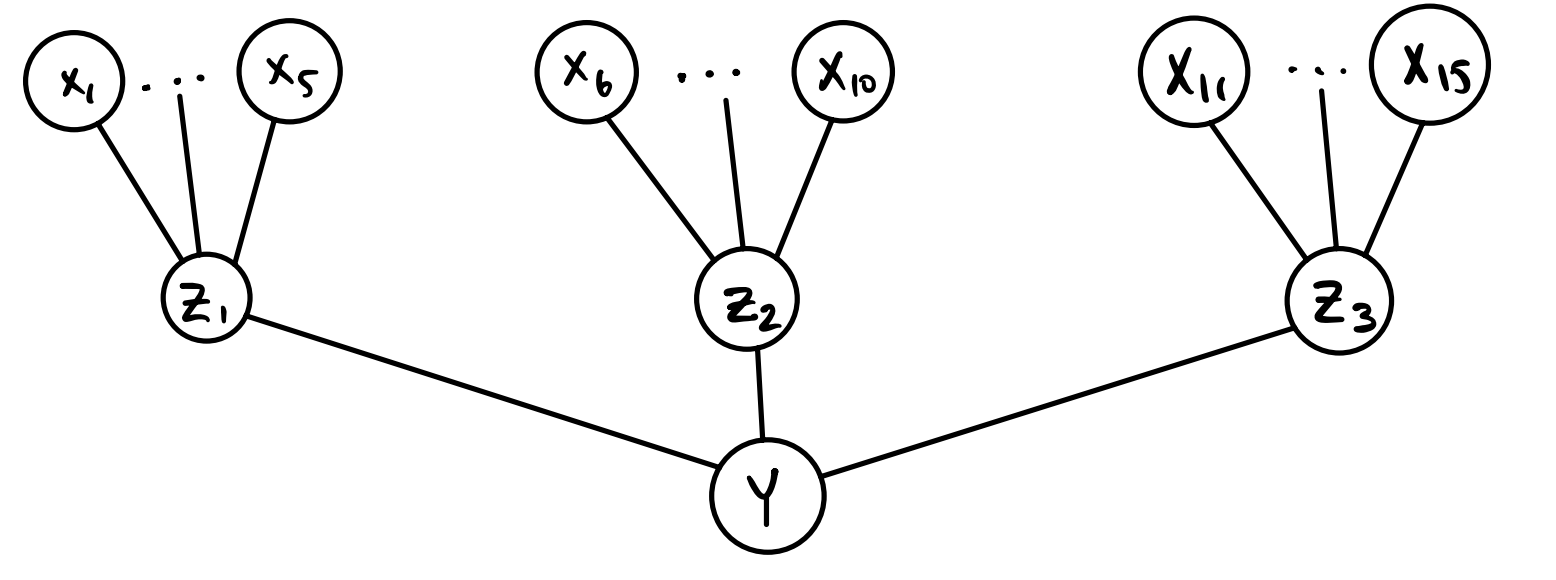
\includegraphics[width=\linewidth]{proposed_model.png}
\end{center}

Let $T$ be the cardinality of the dataset, $x_i$ be the features, $z_i$ be the hidden variables, and $Y \in \{0,1\}$ be whether a second date occurs. We denote $\vec{X^{(i)}} = \{x_{5i-4}, x_{5i-3}, \dots, x_{5i}\}$, $\vec{X} = \{\vec{X}^{(1)},\vec{X}^{(2)},\vec{X}^{(3)}\}$, $\vec{Z} = \{Z_i,Z_2,Z_3\}$.
% We assume x and y to be independent.


\subsection{EM Algorithm}

We want to learn the CPTs using Expectation Maximization.


% \[ P(\vec{X},Y) = \sum_Z P(\vec{X})P(Z|\vec{X})P(Y|Z) \]

\subsubsection{E-step}

% \[
% \begin{aligned}
% P(\vec{Z}|\vec{X},Y)
% &= \frac{P(\vec{X},\vec{Z},Y)}{P(\vec{X},Y)}
% = \frac{P(\vec{X})P(\vec{Z}|\vec{X})P(Y|\vec{Z})}{\sum_{\vec{Z'}}P(\vec{X},\vec{Z'},Y)}
% = \frac{P(\vec{X})P(\vec{Z}|\vec{X})P(Y|\vec{Z})}{\sum_{\vec{Z'}}P(\vec{X})P(\vec{Z'}|\vec{X})P(Y|\vec{Z'})} \\
% &= \frac{P(\vec{Z}|\vec{X})P(Y|\vec{Z})}{\sum_{\vec{Z'}}P(\vec{Z'}|\vec{X})P(Y|\vec{Z'})}
% \end{aligned}
% \]

$$
  \begin{aligned}
    P(\vec{Z} | \vec{X}, Y)
     & =  \frac{P(\vec{Z}, Y | \vec{X})}{P(Y | \vec{X})}
    = \frac{P(\vec{Z} | \vec{X})P(Y | \vec{Z})}{\sum_{\vec{Z'}} P(\vec{Z'}, Y | \vec{X})}                                      \\
     & = \frac{P(Y|\vec{Z})\prod_{i=1}^3P(Z_i|\vec{X}^{(i)})}{\sum_{\vec{Z'}} P(Y|\vec{Z'})\prod_{i=1}^3P(Z'_i|\vec{X}^{(i)})}
  \end{aligned}
$$

$$
  \begin{aligned}
    P(Z_i | \vec{X}, Y) = \sum_{Z_j, j\neq i} P(\vec{Z} | \vec{X}, Y)
  \end{aligned}
$$

\subsubsection{M-step}

% Root nodes:

% \[ P(\vec{X}) \leftarrow \frac{\sum_{i=1}^T P(\vec{X}|\vec{X}_i,Y_i)}{T} = \frac{\sum_{i=1}^T I(\vec{X},\vec{X}_i)}{T} \]

% Nodes with parents:

$$
  \begin{aligned}
    P(Z_i|\vec{X^{(i)}})
     & \leftarrow \frac{\sum_{t=1}^T P(Z_i,\vec{X^{(i)}} | \vec{X}_t, Y_t)}{\sum_{t=1}^T P(\vec{X^{(i)}}| \vec{X}_t, Y_t)}
    = \frac{\sum_{t=1}^T I(\vec{X^{(i)}},  \vec{X^{(i)}_t}) P(Z_i | \vec{X}_t, Y_t)}{\sum_{t=1}^T I(\vec{X^{(i)}},  \vec{X^{(i)}_t})} \\
  \end{aligned}
$$

$$
  \begin{aligned}
    P(Y|\vec{Z})
     & \leftarrow \frac{\sum_{t=1}^T P(Y,\vec{Z} | \vec{X}_t, Y_t)}{\sum_{t=1}^T P(\vec{Z}| \vec{X}_t, Y_t)}
    = \frac{\sum_{t=1}^T I(Y,  Y_t) P(\vec{Z} | \vec{X}_t, Y_t)}{\sum_{t=1}^T P(\vec{Z}| \vec{X}_t, Y_t)}    \\
  \end{aligned}
$$

% \[ P(\vec{Z}|\vec{X}) \leftarrow \frac{\sum_{i=1}^T P(\vec{X},Z|\vec{X}_i,Y_i)}{\sum_{i=1}^TP(\vec{X}|\vec{X}_i,Y_i)} = \frac{\sum_{i=1}^T I(\vec{X},\vec{X}_i) P(\vec{Z}|\vec{X}_i,Y_i)}{\sum_{i=1}^T I(\vec{X},\vec{X}_i)} \]

% \[ P(Y|\vec{Z}) \leftarrow \frac{\sum_{i=1}^T P(Y,\vec{Z}|\vec{X}_i,Y_i)}{\sum_{i=1}^T P(Z|\vec{X}_i,Y_i)} = \frac{\sum_{i=1}^T I(Y,Y_i) P(\vec{Z}|\vec{X}_i,Y_i)}{\sum_{i=1}^T P(Z|\vec{X}_i,Y_i)} \]

\subsubsection{Inference}

\[
  \begin{aligned}
    P(Y=1 \mid \vec{X})
     & = \sum_{\vec{Z}} P(Y=1, \vec{Z} \mid \vec{X}) 
       = \sum_{\vec{Z}} P(\vec{Z} \mid \vec{X}) P(Y = 1 \mid \vec{Z}) \\
     & = \sum_{\vec{Z}} P(Y=1 \mid \vec{Z}) \prod_{i=1}^3 P(Z_i \mid \vec{X}^{(i)})
  \end{aligned}
\]



\subsection{ML algorithm}
\begin{center}
  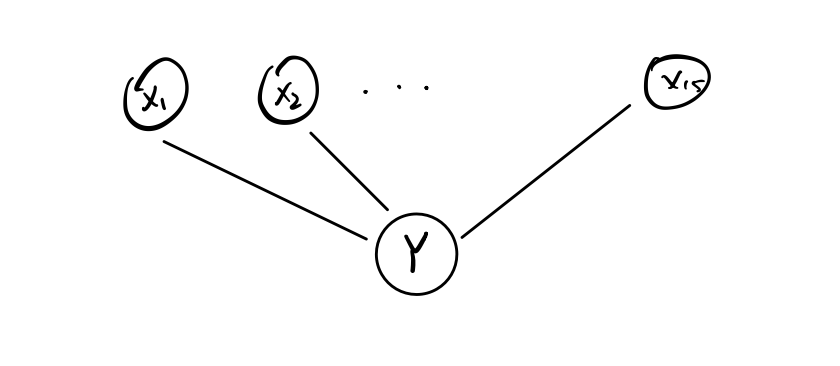
\includegraphics[width=\linewidth]{mle.png}
\end{center}

The second model we used was without hidden states and was another Bayesian network with similar structure as the Noisy-OR model in which all features $\vec{X}$ are parents of $Y$. Since all features are known, we can directly use MLE to estimate our CPTs. Here, let N be the number of samples. Our goal is to find probability of 2nd date $Y$ given all 15 features $\vec{X}$ by calculating $P(Y|\vec{X})$, which is shown below. 
\[
  \begin{aligned}
    &P(Y \mid \vec{X})  = \frac{P(\vec{X}, Y)}{P(\vec{X})} \\
    &\text{where:}\\
    &P(\vec{X}, Y)  = \frac{1}{N} \sum_{n=1}^N I(\vec{x}, \vec{x}^{(n)}) \, I(y, y^{(n)}) \\
    &P(\vec{X})  = \frac{1}{N} \sum_{n=1}^N I(\vec{x}, \vec{x}^{(n)})
  \end{aligned}
\]
\\


\section{Results and Discussion}

In this project, we implemented an 80/20 test–train split, which is common practice in machine learning to assess how the model generalizes to unseen (test) data. We ran two different algorithms, Expectation Maximization (EM) and Maximum Likelihood (ML), each with unbalanced and balanced options on binned and non-binned data. The dataset by itself contains a lot more non-matches than matches, making it heavily unbalanced. To balance it, we randomly sampled the same number of matches and non-matches and ran the model on that new data. The metrics we used to assess model performance were the following: 
\begin{itemize}
    \item\emph{Accuracy:} the percentage of predictions model got right $\frac{TP + TN}{Total}$
    \item\emph{Precision:} percentage of positive predictions that were labeled correctly $\frac{TP}{TP + FP}$
    \item\emph{Recall:} percentage of true positives out of the actual positive instances $\frac{TP}{TP+FN}$
    \item\emph{F1:} metric of precision and recall together 
    \item\emph{ROC AUC Score:} ROC, which plots TPR against FPR, area under curve score
    \item\emph{PR AUC Score:} precision-recall area under curve score 
    \item\emph{Confusion Matrix (using numpy):} count of $\begin{smallmatrix}\text{True Negative (TN)} & \text{False Positive (FP)} \\ \text{False Negative (FN)} & \text{True Positive (TP)}\end{smallmatrix}$ 
\end{itemize}

\begin{table}[ht]
\centering
\caption{Performance of 4 different models on the binned data evaluated using the given metrics.}
\label{tab:model_results}
\begin{tabular}{
  l
  S[table-format=1.3]  % Accuracy
  S[table-format=1.3]  % Precision
  S[table-format=1.3]  % Recall
  S[table-format=1.3]  % F1
  S[table-format=1.3]  % ROC AUC
  S[table-format=1.3]  % PR AUC
  c                    % Confusion matrix
}
\toprule
{Model} & {Accuracy} & {Precision} & {Recall} & {$F_1$} &
{ROC AUC} & {PR AUC} & {Conf. Matrix} \\
\midrule
EM unbalanced & 0.819 & 0.409 & 0.132 & 0.200 & 0.744 & 0.355 &
$\begin{bmatrix} 1334 &  55 \\ 249 &  39 \end{bmatrix}$ \\
EM balanced  & 0.700 & 0.698 & 0.707 & 0.702 & 0.733 & 0.702 &
$\begin{bmatrix}  199 &  88 \\  84 & 203 \end{bmatrix}$ \\
ML unbalanced & 0.526 & 0.163 & 0.429 & 0.236 & 0.493 & 0.171 &
$\begin{bmatrix}  758 & 631 \\ 164 & 123 \end{bmatrix}$ \\
ML balanced  & 0.502 & 0.502 & 0.533 & 0.517 & 0.490 & 0.498 &
$\begin{bmatrix}  135 & 152 \\ 134 & 153 \end{bmatrix}$ \\
\bottomrule
\end{tabular}
\end{table} 

Table 1 shows the performance of each model on the selected metrics using the binned data. The numbers are rounded to three decimal points from the raw result given by running the code. The raw terminal output of the code can be seen in Appendix A.

Even though the unbalanced EM reached the highest accuracy, it performed much worse on the other tested metrics. This is due to the unbalanced nature of the data, where there are significantly more non-matches than matches, making the model more biased toward non-matches. This can be seen in the confusion matrix, which displays an overwhelming amount of negative predictions and a very small number of true positives. This model mostly captures the dominant non-match pattern in the data but misses many actual matches, indicating that it fails to exploit the more meaningful patterns in the data that distinguish successful from unsuccessful dates.

The best overall performing model was the balanced EM. This predictor performs relatively well and is more evenly distributed across all tested metrics. Precision, recall, F1, and PR AUC all increased compared to the unbalanced EM model. The balanced EM performed better at predicting positive outcomes (match) than the unbalanced EM, since the latter can rely on just “guessing” a non-match that heavily overpowers the dataset, making the prediction accurate but not precise. The overall accuracy decrease of balanced EM is a trade-off for improving the other metrics. The balanced EM model appears to capture more accurate predictions of first date success, measured by matching or not matching, compared to the other models we have implemented. However, the confusion matrix still shows a noticeable number of false negatives and false positives, suggesting that our chosen features do not fully explain real-world second date decisions.

The ML model performance was poor compared to the EM algorithm. Both ML implementations performed poorly on the data, producing barely better than chance (0.50) predictions. The unbalanced version yielded low precision, F1, and PR AUC scores, making the balanced implementation seem better. Nonetheless, even the balanced ML produced predictions that can largely be attributed to random guessing. 

After the initial iteration of the project, we decided to try running our models with unbinned data. All the features still maintained discrete values, some values were given a score 0-100 and others a score of 0-10. Previously, the values were attributed into 3 bins, described in the \emph{Dataset Source and Processing} section. Table 2 displays the results of running the four models described above on unbinned data and evaluates them on the same metrics as before.  

\begin{table}[ht]
\centering
\caption{Un-binned data performance.}
\label{tab:model_results}
\begin{tabular}{
  l
  S[table-format=1.3]  % Accuracy
  S[table-format=1.3]  % Precision
  S[table-format=1.3]  % Recall
  S[table-format=1.3]  % F1
  S[table-format=1.3]  % ROC AUC
  S[table-format=1.3]  % PR AUC
  c                    % Confusion matrix
}
\toprule
{Model} & {Accuracy} & {Precision} & {Recall} & {$F_1$} &
{ROC AUC} & {PR AUC} & {Conf. Matrix} \\
\midrule
EM unbalanced & 0.836 & 0.557 & 0.206 & 0.300 & 0.787 & 0.425 &
$\begin{bmatrix} 1342 &  47 \\ 228 &  59 \end{bmatrix}$ \\
EM balanced  & 0.730 & 0.72 & 0.753 & 0.736 & 0.801 & 0.787 &
$\begin{bmatrix}  203 &  84 \\  71 & 216 \end{bmatrix}$ \\
ML unbalanced & 0.507 & 0.183 & 0.544 & 0.274 & 0.517 & 0.182 &
$\begin{bmatrix}  694 & 695 \\ 131 & 156 \end{bmatrix}$ \\
ML balanced  & 0.524 & 0.523 & 0.554 & 0.538 & 0.521 & 0.511 &
$\begin{bmatrix}  142 & 145 \\ 128 & 159 \end{bmatrix}$ \\
\bottomrule
\end{tabular}
\end{table} 

Using the unbinned data, there has been a noticeable increase in performance across the board in almost all of the metrics, except for the accuracy in ML unbalanced. This improvement can be attributed to a general increase of true negative and true positive predictions, which are reflected in the confusion matrices. The general trend still remains: unbalanced EM had the highest accuracy, balanced EM had the best overall performance, the two ML models performed worse, and results from balanced ML are very close to chance. 

Overall, the ML algorithms performed much worse than the EM ones, illustrating that the more robust EM-based model with latent variables generalizes better on unseen data. It can also be seen that balanced implementations consistently outperformed the unbalanced ones, showing the significance of dataset manipulation and balancing. Additionally, in our second implementation, using unbinned data noticeably improved the performance on the given metrics but the originally discovered trends of model performance were maintained.  \\

\section{Conclusion}
In this project, we attempted to predict the probability of a second date based on features derived from three hand-picked traits: attractiveness, intelligence, and sincerity. We constructed a Bayesian Network with hidden variables and applied the EM and ML algorithms to obtain the most accurate prediction of a match. The EM models significantly outperformed the ML ones, and there was notable improvement in balancing the dataset. The balanced EM model performed best overall, giving us the highest and most evenly distributed results on several model assessment metrics. 

Even with these successful predictions, our model’s performance can be improved, as our project had several limitations. First, the original unbalanced nature of the dataset created a strong bias towards non-match predictions. We handled this through randomly sampling the same number of matches as non-matches. This balancing technique proved beneficial for model performance but considerably decreased the amount of data available for us to work with. An improved implementation of this project would use a large, more evenly distributed dataset or more sophisticated methods for handling imbalance. Another limitation is that we hand-picked traits and features that seemed the most relevant. Due to the short timeline of this project, that strategy was the most efficient way to produce a working result. However, this means that there might be other features and traits that are stronger predictors of second date match. Future work should conduct a more in-depth analysis of which features are most significant in forming this prediction. Another avenue for potential extensions is to explore richer networks that are able to capture more nuanced processes that go into match making. Overall, this project is an interesting contribution to exploring how finding love can be made more certain through probabilistic methods. 

\section{Reflections and Contributions}
\textbf{Ekansh Kushwaha}\\ 
For the technical execution, I helped drive the selection of our two final models and outlined the implementation roadmap to ensure our code was structured effectively. I also took ownership of the 'Data Sourcing and Processing' section in our final report. This project was a major confidence builder for me. It bridged the gap between theory and practice, teaching me how to adapt standard classroom models for messy, real-world scenarios. It also sharpened my ability to handle public datasets and reinforced the value of collaborative development. I used Gen AI in parts of the writing process to help convey my thoughts in a more clear and succinct manner.\\

\textbf{Inna Amogolonova}\\
For the report, I take primary ownership over the “Results and Discussion” and the “Conclusion” sections. My other contributions include active participation in team meetings, effective communication in the chat throughout the entire project, and overall edits to the final report. Our team worked well together overall and everyone participated their fair share. This project was helpful in extending my knowledge of the topics we discussed in lecture. As a hands-on learner, application of theory in this way is the most helpful way for me to learn and increase my comprehension of topics that were previously unfamiliar. The topic was interesting and kept me motivated throughout the entire project. Overall, through working on this project, I have gained a deeper understanding that will stick with me much longer than the extent of this class, which I think is very valuable. For future students, I would suggest starting early and getting the majority of the project done by Milestone 2, if possible. This is what my team did and it relieved a lot of stress going into week 10/finals. \\


\textbf{Michael Dai}\\
I performed data analysis and preprocessing on the raw data to fit it to our model’s parameters. The dataset we chose did not require much preparation, as most of it was clean. However, for example, we still had to fix an issue due to spelling errors in the raw data, which was a result of discrepancies between the data’s CSV file and its online description on Kaggle. I wrote some helper functions for running a second test and storing some MLE probabilities. I ran a second test to test model performance given slightly different data. We wanted to observe whether given 2 sets of similar data from the same observation of the sample, what differences can appear. I also edited and proofread the report. I learned that knowing the data’s structure, values, and possible errors is important for reaching good model results and can reduce debugging time. I also learned how to process the raw data into a format the model can understand and how choosing data features can affect model performance. \\

\textbf{Sean Ko}\\
I drew up the Bayesian networks and wrote out the mathematical derivations for the EM algorithm. I was also a part of the group effort to find the problem statement, dataset, and the features our team wanted to use. The derivations and the drawing solidified my understanding of how EM is used in practice and also broadened my view of where Bayesian networks can be applied. What really helped our team find success was early communication and ownership. Everybody played a part and was not shy to voice their opinion / listen to others.\\

\textbf{Zirui You}\\
I developed the model architecture and formulated the experimental design, including comparisons between models with and without hidden states and analyses of balanced versus unbalanced datasets. Additionally, I was responsible for the implementation of the project code and assisted in deriving the EM algorithm’s mathematical formulations. In this project, I learned how important hidden states are when the dataset is limited. Without them, the CPT size explodes to 14,348,907, making it larger than the dataset and impossible to estimate reliably.  Adding 3 hidden states decouples feature dependencies, reduces the CPT size to 737, and significantly improves performance. Although I initially worried that our model was too simple, the hidden-state model still reached about 70\% accuracy and precision on the balanced test set, showing that the methods from this course are genuinely effective for real-world problems.


\section{References}
Khin Yap, J. (2020). Speed dating [Data set]. Kaggle. Retrieved on Nov 19, 2025 from https://www.kaggle.com/datasets/polarbearyap/speed-dating. 


\section{Appendix A: Raw Terminal Output }

\begin{center}
  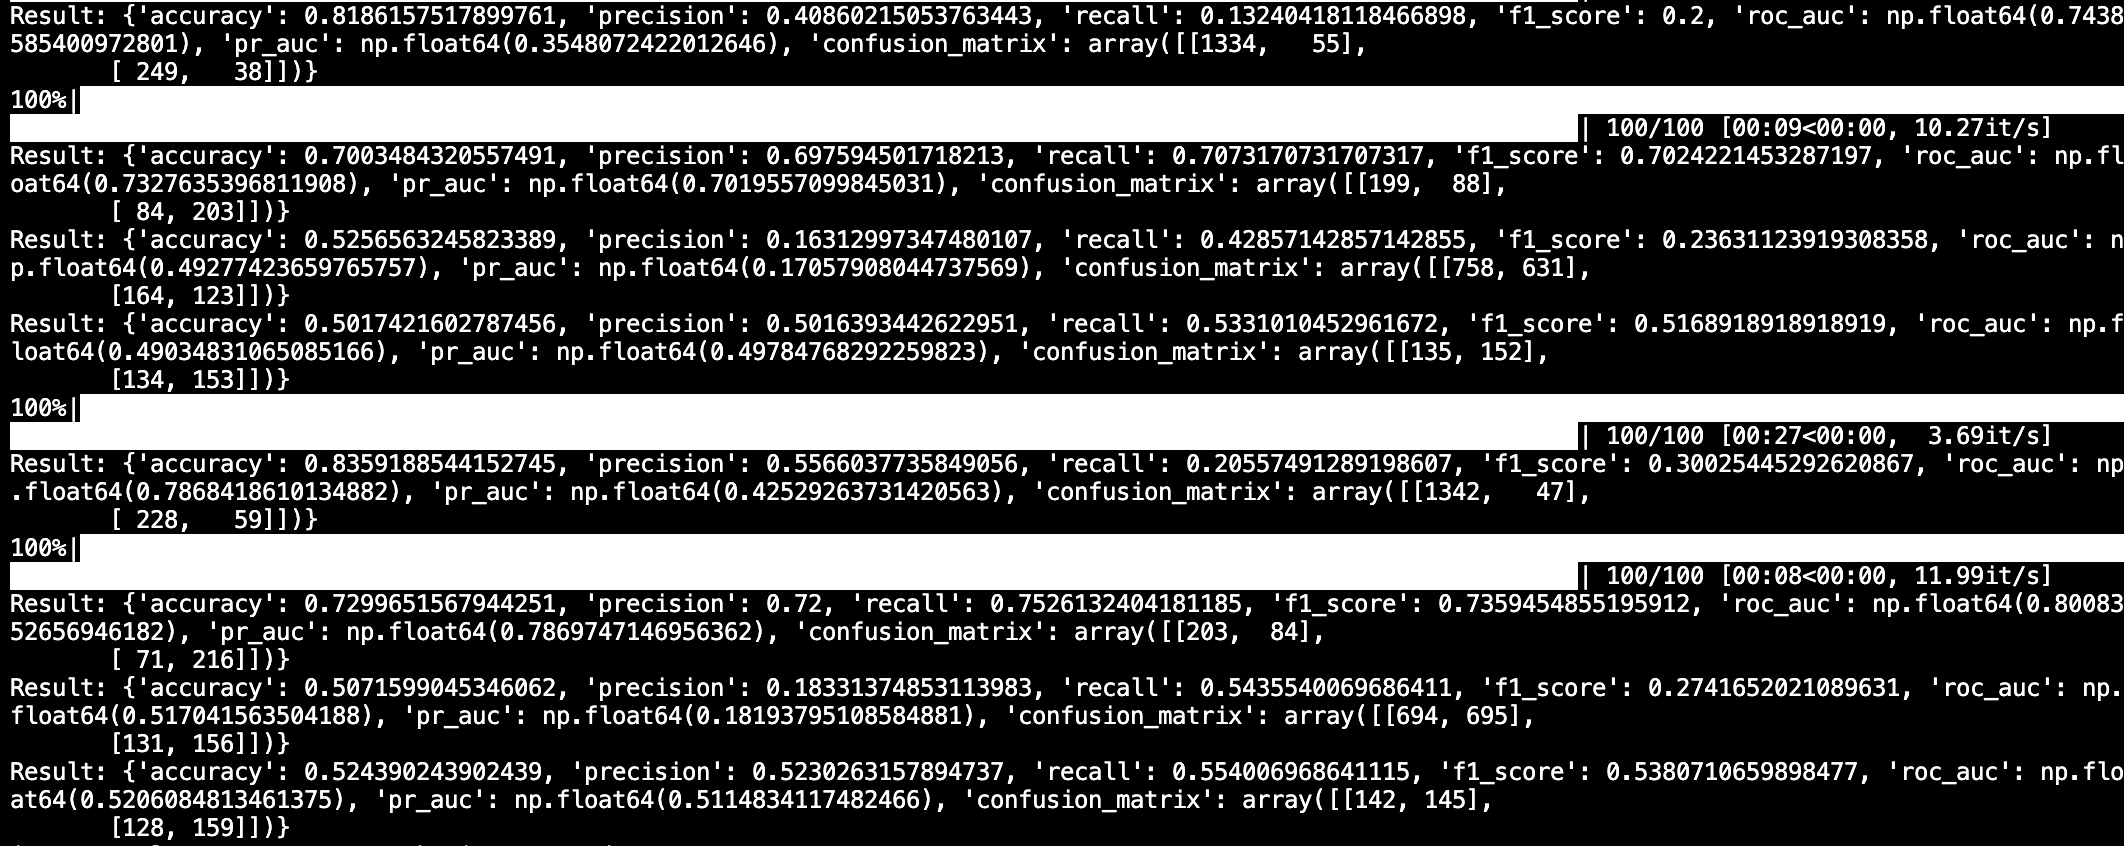
\includegraphics[width=\linewidth]{terminal_output.png}
\end{center}

The model results are displayed in the following order: 
\begin{enumerate}
    \item EM unbalanced binned
    \item EM balanced binned
    \item ML unbalanced binned
    \item ML balanced binned
    \item EM unbalanced unbinned
    \item EM balanced unbinned
    \item ML unbalanced unbinned
    \item ML balanced unbinned
\end{enumerate}
     


\end{document}